% How to draw a Plane intersecting a Cone in LaTeX
% http://latexdraw.com
% 13/10/2019, 11:34
\documentclass{standalone}

\usepackage{tikz}
\usepackage{pgfplots}
\usepgfplotslibrary{colormaps}

\pgfplotsset{compat = newest}

\begin{document}
    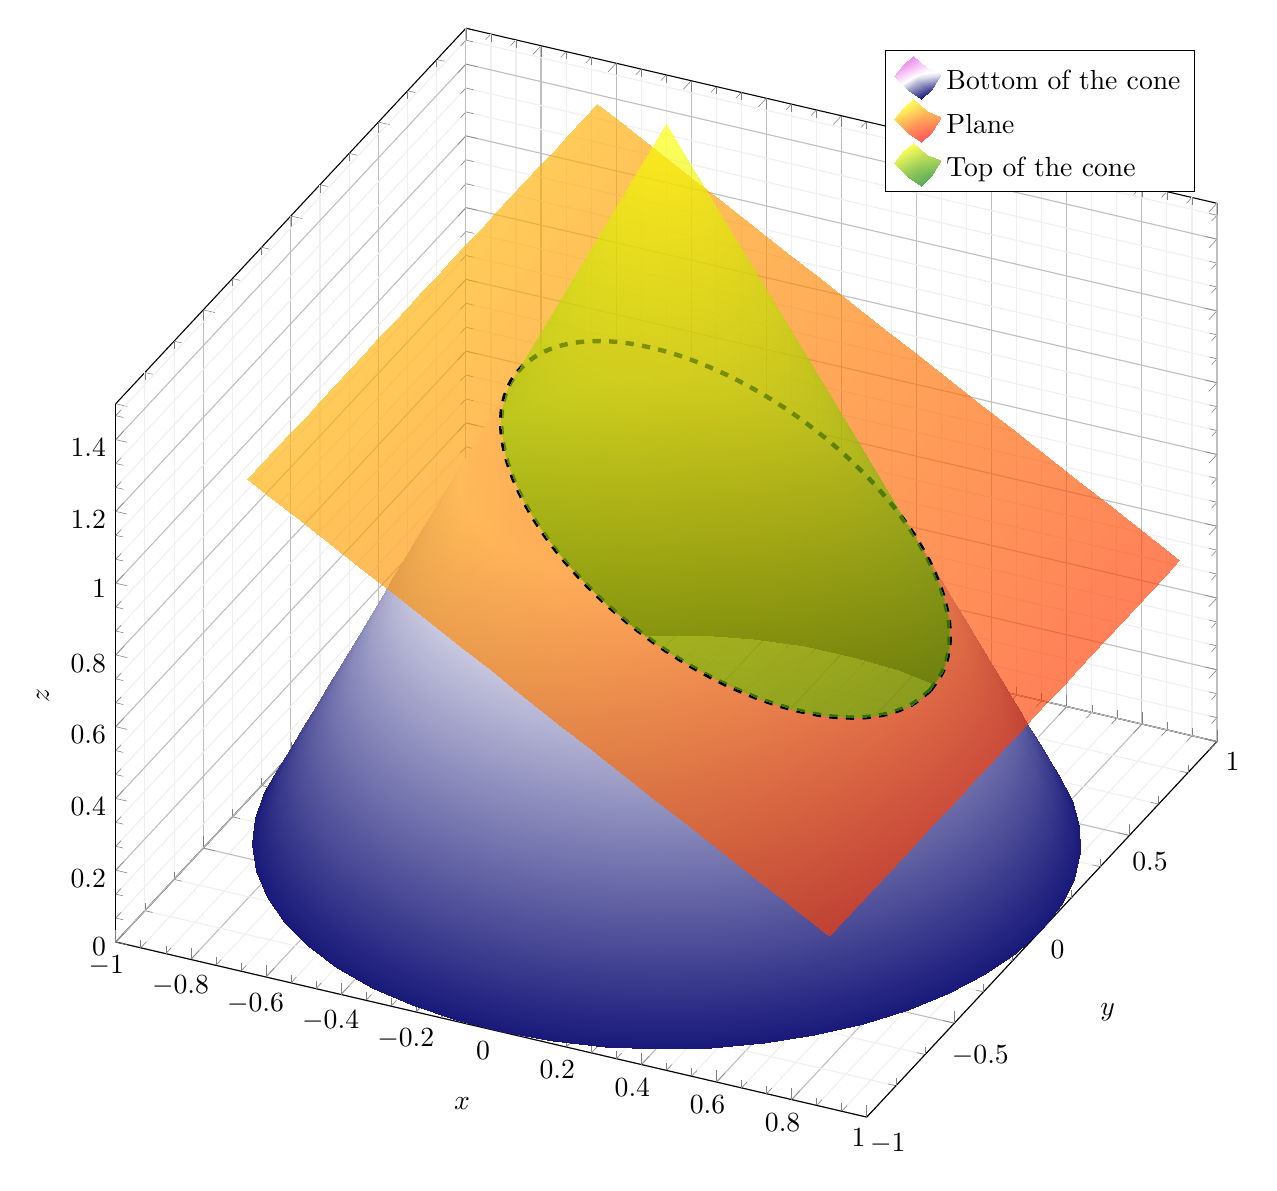
\begin{tikzpicture}
        \begin{axis}[
            axis equal image,
            grid = both,
            minor tick num = 2,
            xlabel = {$x$},
            ylabel = {$y$},
            zlabel = {$z$},
            major grid style = {draw = lightgray},
            minor grid style = {draw = lightgray!25},
            legend cell align={left},
            ymin = -1, ymax = 1,
            xmin = -1, xmax = 1,
            scale = 3,
            zmin = 0, zmax = 1.5,
            z buffer = sort,
        ]
            % bottom of the cone
            \addplot3[
                surf,
                shader = interp,
                samples = 50,
                samples y = 20,
                domain = 0:2*pi,
                domain y = 0:1,
                colormap/violet,
            ]
            (
                {cos(deg(x)) + ((sin(60) /
                (2*sin(60)-cos(60)*cos(deg(x))))*cos(deg(x))-cos(deg(x)))*y},
                {sin(deg(x)) + ((sin(60) /
                (2*sin(60)-cos(60)*cos(deg(x))))*sin(deg(x))-sin(deg(x)))*y},
                {0 + (-2*(sin(60) /
                (2*sin(60)-cos(60)*cos(deg(x))))+2-0)*y}
            );

            % plane
            \addplot3[
                surf,
                shader = interp,
                opacity = 0.65,
                domain = -0.65:0.9,
                domain y = -1:1,
                colormap/redyellow
            ]   {-cos(60)/sin(60)*x+1};

            % ellipse
            \draw[
                samples = 50,
                smooth,
                domain = 0:2*pi,
                variable = \t,
                dashed,
                ultra thick
            ]
            plot (
                {(sin(60) /
                (2*sin(60) - cos(60)*cos(deg(\t))))*cos(deg(\t))},
                {(sin(60) /
                (2*sin(60) - cos(60)*cos(deg(\t))))*sin(deg(\t))},
                {-2*(sin(60) /
                (2*sin(60) - cos(60)*cos(deg(\t))))+2}
            );

            % top of the cone
            \addplot3[
                surf,
                shader = interp,
                samples = 50,
                samples y = 5,
                domain = 0:2*pi,
                domain y = 0:1,
                opacity = 0.65,
                colormap/greenyellow,
            ]
            (
                {0 + ((sin(60) /
                (2*sin(60)-cos(60)*cos(deg(x))))*cos(deg(x))-0)*y},
                {0 + ((sin(60) /
                (2*sin(60)-cos(60)*cos(deg(x))))*sin(deg(x))-0)*y},
                {2 + (-2*(sin(60) /
                (2*sin(60)-cos(60)*cos(deg(x))))+2-2)*y}
            );

            \legend{Bottom of the cone, Plane, Top of the cone}
        \end{axis}
    \end{tikzpicture}
\end{document}
